\documentclass[8pt,a4paper,compress]{beamer}

\usepackage{/home/siyer/lib/slides}

\title{Programming Environment}
\date{}

\newlength{\myMheight}
\settoheight{\myMheight}{M}

\begin{document}
\begin{frame}
\vfill
\titlepage
\end{frame}

\section{Programming Environment}
\begin{frame}[fragile]
\pause

VirtualBox

\pause\bigskip

Linux-based virtual machine (ElementaryOS)

\pause\bigskip

\begin{center}
\visible<4->{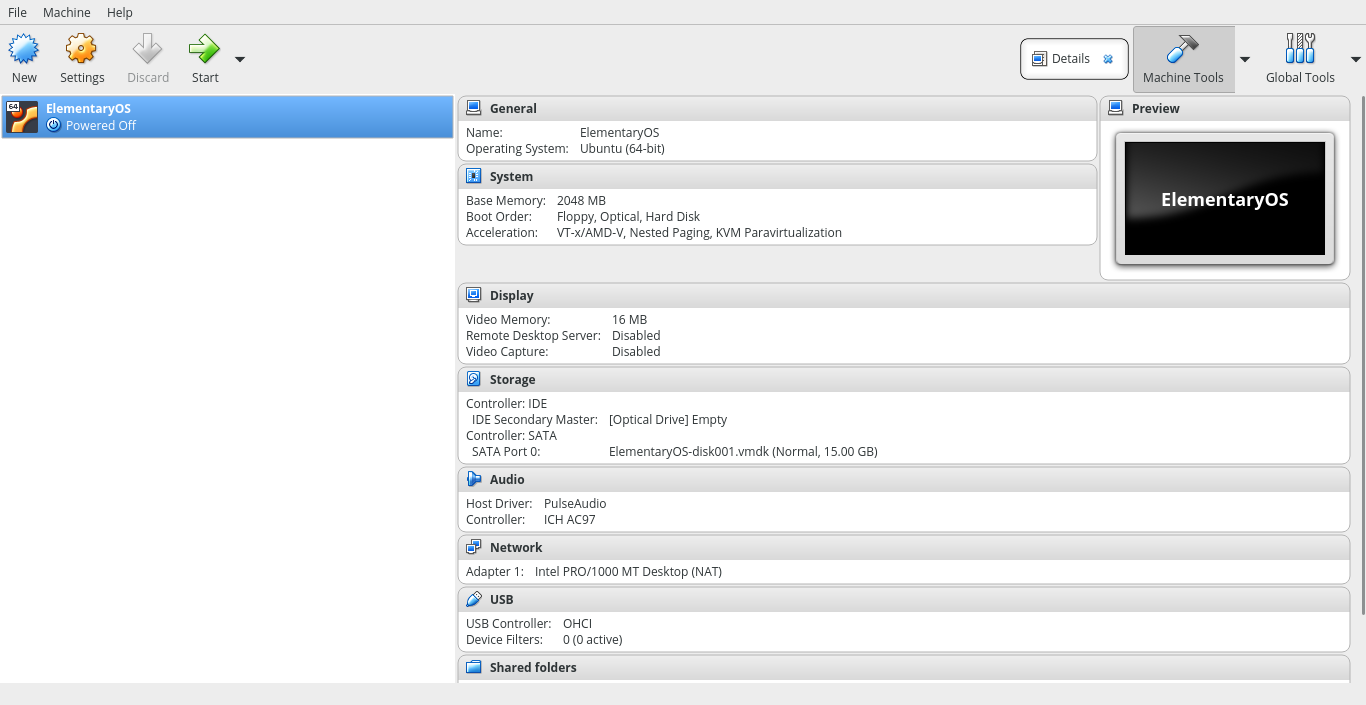
\includegraphics[scale=0.2]{figures/vbox.png}}
\end{center}
\end{frame}

\section{ElementaryOS}
\begin{frame}[fragile]
\pause

Click ``Start'' to start the machine

\pause\bigskip

Login as Uber Student (username \lstinline{student}) with password \lstinline{enigma}

\pause\bigskip

\begin{center}
\visible<4->{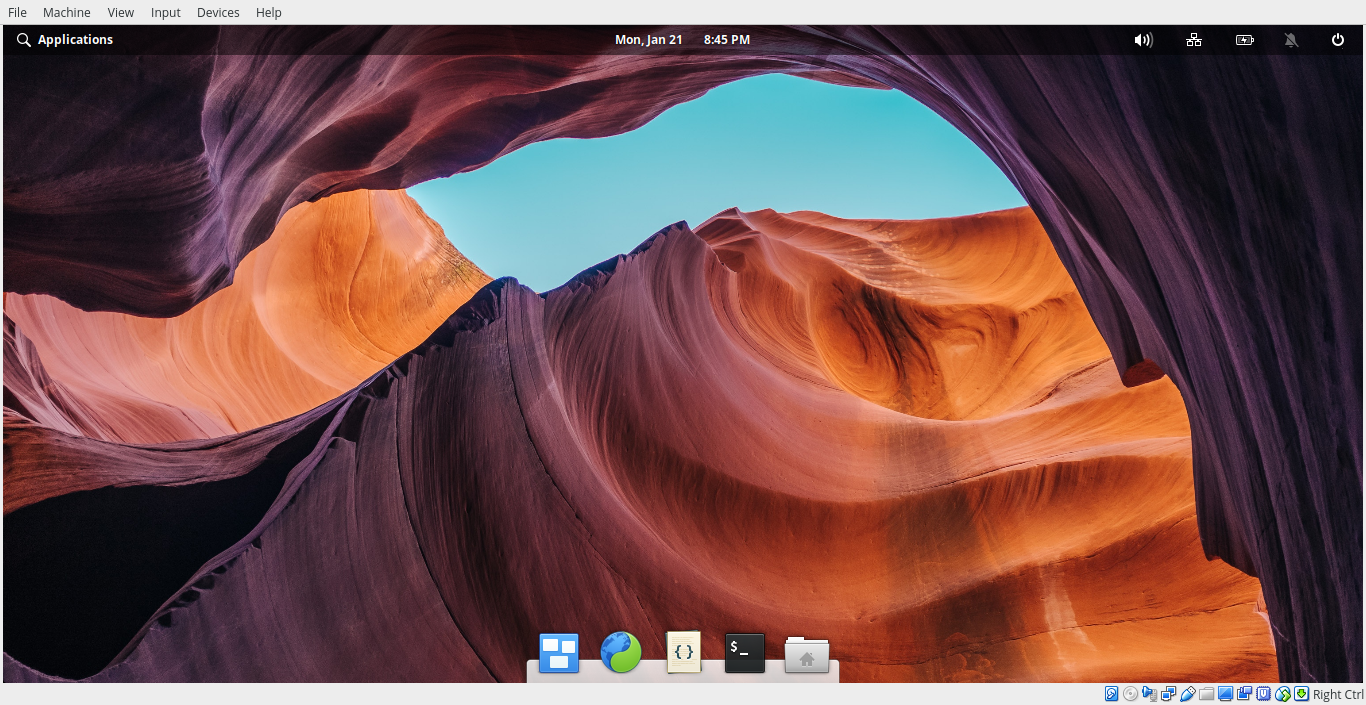
\includegraphics[scale=0.2]{figures/elementaryos.png}}
\end{center}

\pause\bigskip

On the dock: Web Browser \visible<5->{
\includegraphics[height=\myMheight]{figures/web_browser.pdf}}, Editor \visible<5->{
\includegraphics[height=\myMheight]{figures/editor.pdf}}, Terminal \visible<5->{
\includegraphics[height=\myMheight]{figures/terminal.pdf}}, File manager \visible<5->{
\includegraphics[height=\myMheight]{figures/file_manager.pdf}}

\pause\bigskip

To stop the machine, click \visible<6->{
\includegraphics[height=\myMheight]{figures/shutdown.pdf}} and select ``Shut Down...''
\end{frame}

\section{Editing Files}
\begin{frame}[fragile]
\pause

Use editor \visible<2->{
\includegraphics[height=\myMheight]{figures/editor.pdf}}

\smallskip

\begin{center}
\visible<2->{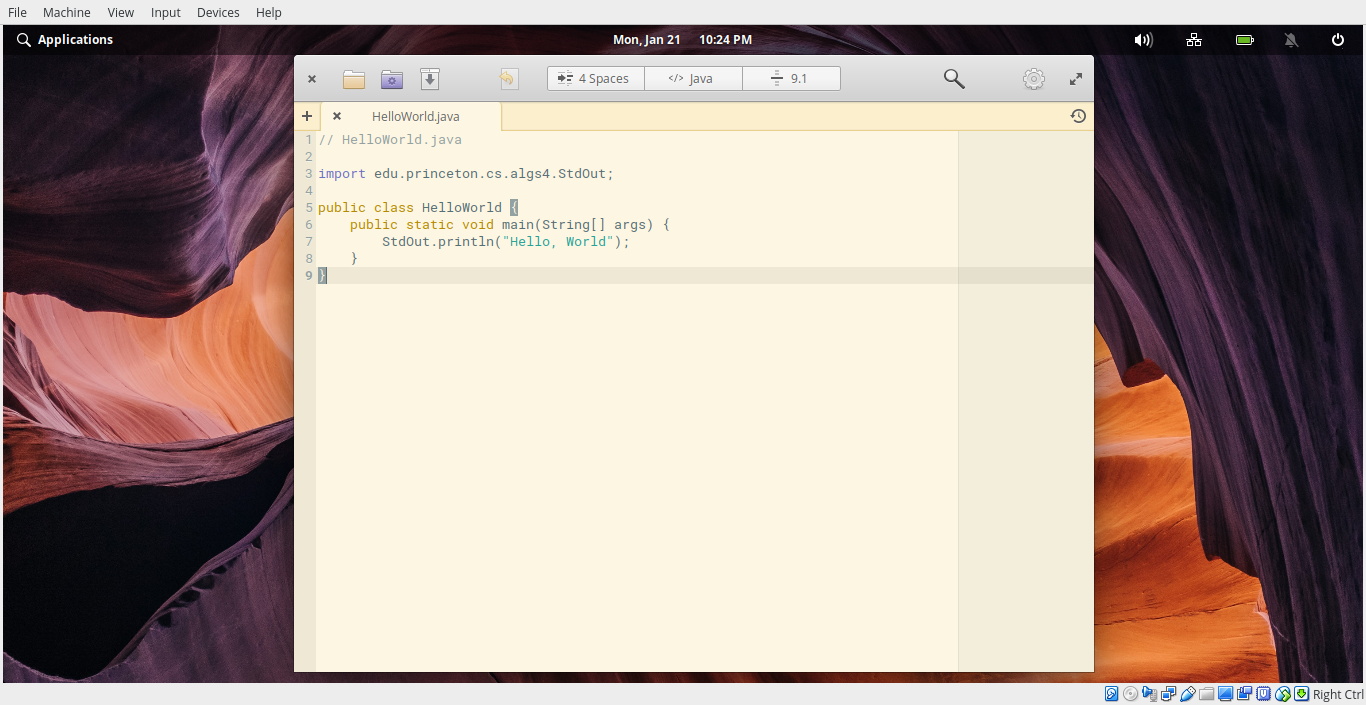
\includegraphics[scale=0.2]{figures/editing.png}}
\end{center}
\end{frame}

\section{Navigating the File System}
\begin{frame}[fragile]
\pause

Use file manager \visible<2->{
\includegraphics[height=\myMheight]{figures/file_manager.pdf}} and terminal \visible<2->{
\includegraphics[height=\myMheight]{figures/terminal.pdf}}

\smallskip

\begin{center}
\visible<2->{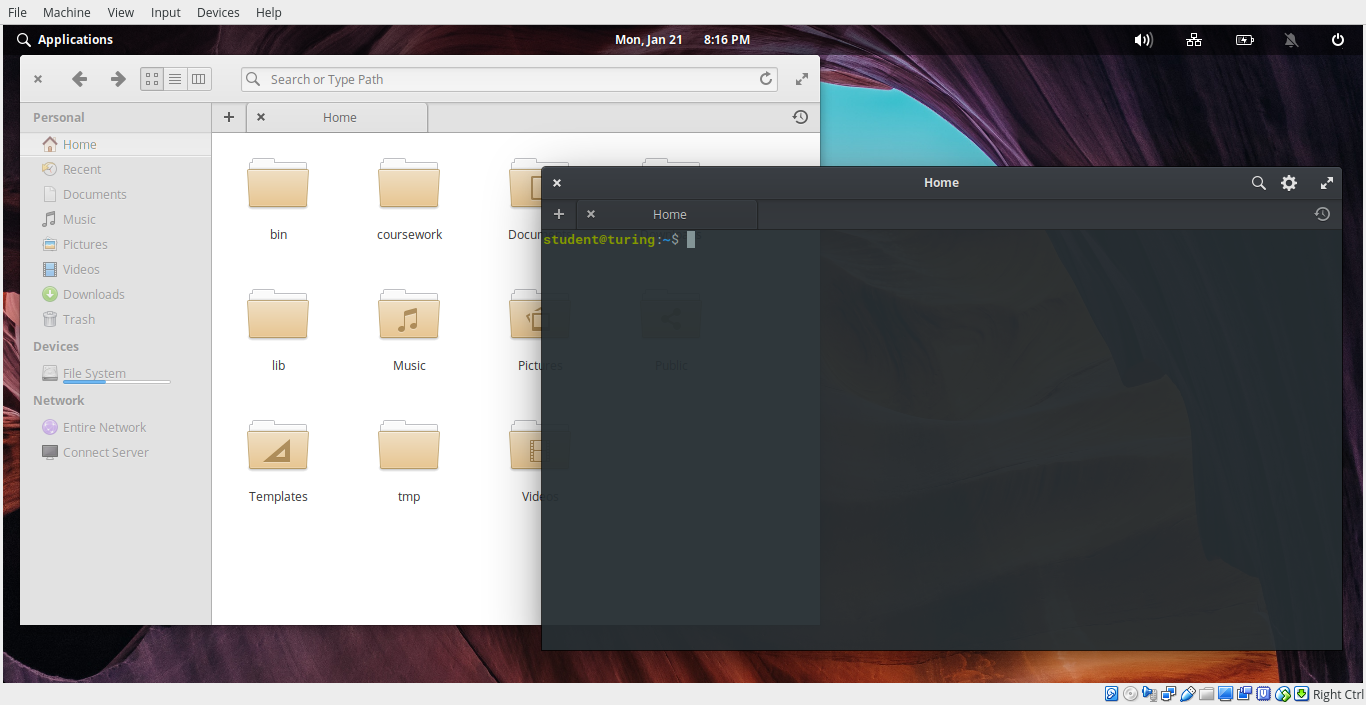
\includegraphics[scale=0.2]{figures/filesystem.png}}
\end{center}
\end{frame}

\section{Obtaining a Project}
\begin{frame}[fragile]
\pause

Launch terminal (opens in \lstinline{/home/student} by default)

\pause\bigskip

Change directory to \lstinline{coursework}

\begin{tcolorbox}[enhanced,drop shadow southwest,sharp corners,size=fbox,colback=black]
\begin{lstlisting}[style=terminal]
$ cd coursework
\end{lstlisting}
\end{tcolorbox}

\pause\bigskip

Download the project (eg, Project 1)

\begin{tcolorbox}[enhanced,drop shadow southwest,sharp corners,size=fbox,colback=black]
\begin{lstlisting}[style=terminal]
$ wget https://swamiiyer.net/cs210/project1.zip
\end{lstlisting}
\end{tcolorbox}

\pause\bigskip

Extract the downloaded zip file

\begin{tcolorbox}[enhanced,drop shadow southwest,sharp corners,size=fbox,colback=black]
\begin{lstlisting}[style=terminal]
$ unzip project1.zip
\end{lstlisting}
\end{tcolorbox}

\pause\bigskip

List current directory

\begin{tcolorbox}[enhanced,drop shadow southwest,sharp corners,size=fbox,colback=black]
\begin{lstlisting}[style=terminal]
$ ls
project1 project1.zip
\end{lstlisting}
\end{tcolorbox}

\pause\bigskip

Remove the zip file

\begin{tcolorbox}[enhanced,drop shadow southwest,sharp corners,size=fbox,colback=black]
\begin{lstlisting}[style=terminal]
$ rm project1.zip
\end{lstlisting}
\end{tcolorbox}
\end{frame}

\section{Working on the Project}
\begin{frame}[fragile]
\pause

Change to the project directory

\begin{tcolorbox}[enhanced,drop shadow southwest,sharp corners,size=fbox,colback=black]
\begin{lstlisting}[style=terminal]
$ cd project1
\end{lstlisting}
\end{tcolorbox}

\pause\bigskip

We are now under \lstinline{/home/student/coursework/project1}

\pause\bigskip

Compile a program (eg, \lstinline{PercolationStats.java})

\begin{tcolorbox}[enhanced,drop shadow southwest,sharp corners,size=fbox,colback=black]
\begin{lstlisting}[style=terminal]
$ javac PercolationStats.java
\end{lstlisting}
\end{tcolorbox}

\pause\bigskip

Run a program (eg, \lstinline{PercolationStats.class})

\begin{tcolorbox}[enhanced,drop shadow southwest,sharp corners,size=fbox,colback=black]
\begin{lstlisting}[style=terminal]
$ java PercolationStats 100 1000
\end{lstlisting}
\end{tcolorbox}

\pause\bigskip

Check a program (eg, \lstinline{PercolationStats.java}) for coding style

\begin{tcolorbox}[enhanced,drop shadow southwest,sharp corners,size=fbox,colback=black]
\begin{lstlisting}[style=terminal]
$ check_style PercolationStats.java
\end{lstlisting}
\end{tcolorbox}
\end{frame}

\begin{frame}[fragile]
\pause

Test your solutions for particular exercises/problems (eg, Exercise 1 and Problem 2)

\begin{tcolorbox}[enhanced,drop shadow southwest,sharp corners,size=fbox,colback=black]
\begin{lstlisting}[style=terminal]
$ python3 run_tests.py -v Exercise1 Problem2
\end{lstlisting}
\end{tcolorbox}

\pause\bigskip

Test your solutions for all exercises/problems

\begin{tcolorbox}[enhanced,drop shadow southwest,sharp corners,size=fbox,colback=black]
\begin{lstlisting}[style=terminal]
$ python3 run_tests.py -v
\end{lstlisting}
\end{tcolorbox}

\pause\bigskip

Use web browser \visible<4->{
\includegraphics[height=\myMheight]{figures/web_browser.pdf}} to sign on to Gradescope and upload your project files
\end{frame}
\end{document}
